% ============================================================
% IC_TORS'26 / journal-development master
% VALIDATING SHAP-DERIVED DECISION WEIGHTS
% ============================================================
% WORKING MANUSCRIPT RULES
% - No fabricated numerical results.
% - The protocol is pre-specified and version controlled; do not call it
%   "preregistered" unless it is actually deposited in a registry.
% - Set \resultsavailabletrue only after the computational pipeline has
%   generated the referenced result files.
% - Keep \anonymoustrue for double-blind review; switch to false only for
%   camera-ready/submission formats that permit author identification.
% ============================================================

\documentclass[runningheads]{llncs}

\usepackage[T1]{fontenc}
\usepackage[utf8]{inputenc}
\usepackage{graphicx}
\usepackage{amsmath,amssymb,amsfonts}
\usepackage{booktabs}
\usepackage{array}
\usepackage{tabularx}
\usepackage{tikz}
\usetikzlibrary{arrows.meta,positioning}
\usepackage{hyperref}

\hypersetup{hidelinks}

\newif\ifanonymous
\anonymoustrue

\newif\ifresultsavailable
\resultsavailablefalse

\newcommand{\SHAP}{SHAP}
\newcommand{\XGB}{XGBoost}
\newcommand{\MOORA}{MOORA}
\newcommand{\TOPSIS}{TOPSIS}
\newcommand{\CRITIC}{CRITIC}
\newcommand{\Oracle}{\mathrm{Oracle}}
\newcommand{\E}{\mathbb{E}}
\newcommand{\I}{\mathbb{I}}
\newcommand{\clip}{\operatorname{clip}}
\newcommand{\eps}{\varepsilon}

\begin{document}
\emergencystretch=1.5em

\title{Validating SHAP-Derived Decision Weights for ITS Prioritisation under Data Scarcity: A Controlled XAI--MCDM Benchmark}
\titlerunning{Validating SHAP-Derived Decision Weights}

\ifanonymous
\author{Anonymous Author(s)}
\authorrunning{Anonymous Author(s)}
\institute{Anonymous institution(s)}
\else
\author{Mohamed Yassine Neifar\inst{1,2} \and
Nadir Farhi\inst{1} \and
Ahmed Frikha\inst{2}}
\authorrunning{Neifar et al.}
\institute{Universit\'e Gustave Eiffel, COSYS--GRETTIA,
14--20 Boulevard Newton, Cit\'e Descartes, Champs-sur-Marne,
F-77447 Marne-la-Vall\'ee Cedex 2, France
\and
Institut Sup\'erieur de Gestion Industrielle de Sfax (ISGIS), OLID,
University of Sfax, Route de l'A\'eroport km 4, BP 1099,
Sfax 3038, Tunisia\\
\email{yessine.neifar.imsil@isgis.usf.tn}}
\fi

\maketitle

\begin{abstract}
Feature-attribution scores are increasingly reused as data-driven criterion weights in
multi-criteria decision-making (MCDM), although predictive importance is neither a causal
effect nor a stakeholder preference. This paper tests when such a conversion preserves
 decision quality. We construct a controlled Intelligent Transportation Systems (ITS)
benchmark in which six deployment alternatives are evaluated on ten technology-neutral
criteria across repeated synthetic contexts. A monotone nonlinear oracle with pairwise
interactions provides an internally known decision reference. XGBoost is trained on a noisy
outcome whose noise level is scaled to the oracle signal, and interventional TreeSHAP values
are converted into global surrogate weights. The oracle is explained with the same
interventional functional, using a closed-form Shapley solution for the pairwise structure.
SHAP is compared with non-negative Ridge, permutation importance, CRITIC, entropy and equal
weights, while Direct-XGBoost ranking and random weights provide diagnostic references.
The design varies data scarcity, predictor dependence, relative noise and interaction
strength, and evaluates attribution recovery, Kendall rank agreement and normalized decision
regret. The contribution is not a new SHAP--MCDM combination, but a controlled audit of the
prediction--attribution--weight-compression--decision chain and the conditions under which
that chain remains reliable.

\keywords{Explainable AI \and SHAP \and Multi-Criteria Decision-Making \and
Intelligent Transportation Systems \and Decision Fidelity}
\end{abstract}

% ============================================================
\section{Introduction}
\label{sec:intro}
% ============================================================

Urban transport agencies often need to prioritise Intelligent Transportation Systems (ITS)
when investment capacity and detailed operational evidence are limited. Candidate
interventions differ in mobility, reliability, safety, environmental performance, user
benefits, infrastructure requirements and lifecycle burden, making the problem naturally
multi-criteria. A persistent difficulty is the provenance of criterion weights. Expert-derived
weights encode preferences; objective methods such as CRITIC and entropy encode properties of
the decision data; supervised approaches instead exploit an external outcome and therefore
capture outcome-conditioned predictive relevance \cite{diakoulaki1995critic,shannon1948}.

Recent studies have begun using explainable artificial intelligence (XAI) to derive MCDM
weights. Ciano and Ferrara integrate attribution methods with several MCDM procedures
\cite{ciano2025xaimcdm}, while Demir et al. combine SHAP-based feature information with
MULTIMOORA \cite{demir2025shapmultimoora}. ML--MCDM integration has also appeared in
transportation decision support \cite{zakeri2024mlmcdm}. Consequently, merely chaining
``XGBoost--SHAP--MCDM'' is no longer a defensible novelty claim.

The unresolved issue is more fundamental. A SHAP value explains a predictive model under a
specified value function and background distribution; it does not automatically represent a
causal effect, a decision-maker preference or a marginal rate of substitution
\cite{janzing2020causal,aas2021dependent}. Kumar et al. further show that Shapley-based
feature-importance interpretations require care about the explanation question itself
\cite{kumar2020shapleyproblems}. Thus, converting predictive attributions into global MCDM
weights should be treated as a hypothesis to test rather than an established principle.

This paper asks four questions: (RQ1) how data scarcity affects predictive recovery of a known
nonlinear utility; (RQ2) how accurately TreeSHAP global weights recover oracle interventional
Shapley importance under dependence, noise and interactions; (RQ3) whether attribution
fidelity survives global-weight compression and downstream MCDM; and (RQ4) whether SHAP adds
value beyond simpler supervised and unsupervised weighting methods, and where its validity
boundaries lie.

The contribution is threefold. First, we extend controlled XAI benchmarking downstream from
attribution fidelity to ranking fidelity and decision regret. Second, we compare SHAP against
both supervised and unsupervised weighting families while adding a Direct-XGBoost decision
reference that reveals information lost by global-weight compression. Third, we use a paired,
context-grouped factorial design with signal-relative noise, dependence and interaction stress
tests, together with bootstrap and distribution-shift analyses. The identity of the top-ranked
ITS is not the scientific objective.

% ============================================================
\section{Related Work and Contribution Boundary}
\label{sec:related}
% ============================================================

\subsection{Predictive Attribution, Global Importance and Decision Weighting}

SHAP provides additive feature attributions grounded in cooperative game theory
\cite{lundberg2017shap}; TreeSHAP makes these computations efficient for tree ensembles
\cite{lundberg2020trees}. Dependence matters because different feature-removal functionals
answer different questions \cite{janzing2020causal,aas2021dependent}. This study therefore
uses an explicit \emph{interventional} functional for both the oracle and the learned tree
model.

A related global perspective is SAGE, which defines Shapley-based global importance through
predictive loss rather than prediction-level attribution \cite{covert2020sage}. SAGE is
important conceptually, but it targets a different functional from the interventional
prediction-level oracle used here; it is therefore discussed as related global-importance work
rather than treated as a direct estimator of the same oracle weights.

Sudakov et al. study regression-based recovery of synthetic reference criterion weights and
report strong Ridge performance in their setting \cite{sudakov2026weights}. Their benchmark
shows that automated weight recovery itself is already an active research direction. The
present study differs by defining the reference through interventional attribution of a known
nonlinear utility, by explicitly varying dependence and interaction strength, and by propagating
weight-recovery error into downstream MCDM ranking and decision regret.

\subsection{Synthetic XAI Benchmarks}

Synthetic ground-truth XAI benchmarking is not claimed as novel. XAI-Bench provides
configurable synthetic datasets for evaluating attribution methods against quantities such as
ground-truth Shapley values \cite{liu2021xaibench}. OpenXAI provides a broader framework for
systematic evaluation of post-hoc explanations and includes a flexible synthetic generator
\cite{agarwal2022openxai}. XAI-Units pairs synthetic datasets with models whose internal
mechanisms are deliberately controlled \cite{lee2025xaiunits}. These works mainly ask whether
an explanation method recovers a known or controlled explanation structure. Our question begins
one step later: whether that attribution structure remains decision-faithful after it is
compressed into one global weight vector and passed through MCDM.

\subsection{Permutation Importance under Dependence}

Permutation importance is included because it is a supervised, model-dependent comparator.
However, unrestricted permutation can push observations into sparse or unsupported regions of
the feature space when predictors are dependent \cite{hooker2021permutation}. We therefore use
context-block permutation and interpret the high-dependence cells cautiously; poor permutation
importance under strong dependence is not treated automatically as evidence that SHAP is
valid.

% ============================================================
\section{Controlled ITS Benchmark}
\label{sec:benchmark}
% ============================================================

\subsection{Alternatives and Criteria}

The benchmark compares six deployment packages at a common first-stage prioritisation level
(Table~\ref{tab:alternatives}). Broad umbrella strategies are excluded. V2X is deliberately
restricted to cooperative safety services so that it does not subsume adaptive signal timing or
transit-priority functions. The set is representative of deployable TSMO/ITS strategy families
rather than an empirical technology inventory for a specific city
\cite{fhwa2016corridors,fhwa2017atm,usdotv2x}.

\begin{table}[t]
\centering
\caption{ITS alternatives used in the controlled benchmark.}
\label{tab:alternatives}
\small
\begin{tabularx}{\linewidth}{@{}c l X@{}}
\toprule
\textbf{ID} & \textbf{Alternative} & \textbf{Operational scope}\\
\midrule
$A_1$ & ATSC & Adaptive phase, split, offset or cycle decisions.\\
$A_2$ & TSP & Transit-priority requests and signal responses.\\
$A_3$ & TIDM & Incident detection, verification, response and recovery.\\
$A_4$ & RMTI--DRG & Real-time multimodal information and dynamic route guidance.\\
$A_5$ & V2X--CS & Cooperative safety warnings; adaptive signal timing and TSP excluded.\\
$A_6$ & DSM & Dynamic regulatory/advisory speed management and harmonisation.\\
\bottomrule
\end{tabularx}
\end{table}

Ten technology-neutral criteria are used (Table~\ref{tab:criteria}). The original lifecycle
burden criterion is a cost; all other criteria are benefits.

\begin{table}[t]
\centering
\caption{Technology-neutral evaluation criteria.}
\label{tab:criteria}
\small
\begin{tabularx}{\linewidth}{@{}c X c@{}}
\toprule
\textbf{Code} & \textbf{Criterion} & \textbf{Original direction}\\
\midrule
$C_1$ & Mobility-efficiency improvement & Benefit\\
$C_2$ & Travel-time reliability improvement & Benefit\\
$C_3$ & Person-throughput improvement & Benefit\\
$C_4$ & Safety-surrogate improvement & Benefit\\
$C_5$ & Non-recurring-congestion resilience & Benefit\\
$C_6$ & Environmental-efficiency improvement & Benefit\\
$C_7$ & User and accessibility benefit & Benefit\\
$C_8$ & Infrastructure and data readiness & Benefit\\
$C_9$ & Interoperability and scalability & Benefit\\
$C_{10}$ & Annualised lifecycle deployment burden & Cost\\
\bottomrule
\end{tabularx}
\end{table}

The structural capability mask in Table~\ref{tab:mask} defines functional pathways, not field
impact magnitudes. Direct (D), indirect (I) and negligible (0) pathways only determine broad
response-amplitude bands.

\begin{table}[t]
\centering
\caption{Pre-specified structural capability mask. D = direct, I = indirect, 0 = no primary pathway.}
\label{tab:mask}
\scriptsize
\begin{tabular}{@{}lccccccc ccc@{}}
\toprule
 & $C_1$ & $C_2$ & $C_3$ & $C_4$ & $C_5$ & $C_6$ & $C_7$ & Ready & Interop. & Burden\\
\midrule
ATSC      & D & D & D & I & I & I & I & M   & H & M\\
TSP       & I & D & D & I & 0 & I & D & M   & H & L--M\\
TIDM      & I & D & I & D & D & I & I & M   & H & M\\
RMTI--DRG & I & I & I & I & D & I & D & L--M& H & L--M\\
V2X--CS   & I & I & 0 & D & I & I & I & H   & H & H\\
DSM       & D & D & I & D & D & I & I & M--H& H & M--H\\
\bottomrule
\end{tabular}
\end{table}

\subsection{Context Generation with Common Random Numbers}

Each context contains five latent factors
\begin{equation}
\mathbf h_s=(h_{D,s},h_{I,s},h_{T,s},h_{E,s},h_{R,s}),
\label{eq:latent}
\end{equation}
representing demand, incident pressure, transit/person movement, environmental sensitivity and
infrastructure readiness. To obtain an equicorrelated Gaussian copula while pairing the
correlation conditions, generate
$z_{0,s},z_{1,s},\ldots,z_{5,s}\overset{iid}{\sim}\mathcal N(0,1)$ and set
\begin{equation}
\tilde h_{k,s}^{(\rho)}
=\sqrt{\rho}\,z_{0,s}+\sqrt{1-\rho}\,z_{k,s},
\qquad
h_{k,s}^{(\rho)}=\Phi(\tilde h_{k,s}^{(\rho)}).
\label{eq:crn}
\end{equation}
The same base normals are reused for all $\rho$ levels. The opportunity functions for the
first seven criteria are
\begin{align}
o_{s1}&=h_D, &
o_{s2}&=0.60h_D+0.40h_I, &
o_{s3}&=0.60h_D+0.40h_T, \label{eq:opp1}\\
o_{s4}&=0.50h_D+0.50h_I, &
o_{s5}&=h_I, &
o_{s6}&=0.60h_D+0.40h_E, \label{eq:opp2}\\
o_{s7}&=0.40h_D+0.60h_T. \label{eq:opp3}
\end{align}

For $j\le7$, the response amplitude is sampled once per replication seed:
\begin{equation}
\delta_{aj}\sim
\begin{cases}
0, & M_{aj}=0,\\
\mathcal U(0.05,0.20), & M_{aj}=I,\\
\mathcal U(0.20,0.40), & M_{aj}=D,
\end{cases}
\label{eq:effectbands}
\end{equation}
and the criterion score is
\begin{equation}
x_{asj}=\clip\!\left(\delta_{aj}o_{sj}^{\nu_j}+\sigma_x\xi_{asj},0,1\right),
\quad \nu_j=1,\quad \sigma_x=0.02,
\label{eq:responses}
\end{equation}
where $\xi_{asj}\sim\mathcal N(0,1)$ is also reused across factor levels.

Deployment classes use $L\sim U(0.25,0.40)$, $M\sim U(0.45,0.60)$ and
$H\sim U(0.65,0.80)$; compound classes are equal-probability mixtures of their component
classes. With readiness requirement $r_a$, interoperability parameter $\iota_a$ and base
burden $\kappa_a$,
\begin{align}
x_{as8}&=\clip\!\left(1-\max(0,r_a-h_{R,s})+\eta_{as8},0,1\right), \label{eq:c8}\\
x_{as9}&=\clip\!\left(\iota_a+0.10h_{R,s}+\eta_{as9},0,1\right), \label{eq:c9}\\
x_{as,10}&=\clip\!\left(\kappa_a+0.20(1-h_{R,s})r_a+\eta_{as,10},0,1\right). \label{eq:c10}
\end{align}
The one-sided $C_8$ shortfall avoids penalising a context for exceeding a technology's readiness
requirement.

All criteria are then placed on one higher-is-better orientation:
\begin{equation}
g_{asj}=x_{asj}\;(j\le9),
\qquad
g_{as,10}=1-x_{as,10}.
\label{eq:orientation}
\end{equation}
This same representation is used by supervised learning, objective weighting and the primary
MCDM aggregation, eliminating an orientation mismatch between weight estimation and ranking.

\subsection{Oracle Utility and Signal-Relative Noise}

Define the monotone nonlinear transform
\begin{equation}
q_j(g)=\frac{\log(1+\zeta_j g)}{\log(1+\zeta_j)},
\qquad \zeta_j=2.
\label{eq:qtransform}
\end{equation}
The primary oracle uses the heterogeneous coefficient vector
\begin{equation}
\boldsymbol\alpha
=(0.11,0.04,0.05,0.07,0.10,0.14,0.12,0.16,0.08,0.13),
\qquad \sum_j\alpha_j=1,
\label{eq:alpha}
\end{equation}
obtained by a one-time pre-specified permutation (design seed 73001) of the multiset
$(0.16,0.14,0.13,0.12,0.11,0.10,0.08,0.07,0.05,0.04)$. The fixed mapping introduces
heterogeneity without assigning large coefficients to criteria because of a desired ITS outcome.

The interaction graph is
\begin{equation}
\mathcal E=\{(1,2),(3,7),(4,5),(6,10),(8,9)\},
\qquad \beta_{jk}=0.20.
\label{eq:interactions}
\end{equation}
The oracle utility is
\begin{equation}
U_{as}^{\star}
=
\frac{
\sum_{j=1}^{10}\alpha_j q_j(g_{asj})
+\lambda\sum_{(j,k)\in\mathcal E}\beta_{jk}q_j(g_{asj})q_k(g_{ask})
}{1+\lambda}.
\label{eq:oracle}
\end{equation}
The oracle is an internally specified benchmark reference, not a causal ground truth, stakeholder
preference function or social-welfare model.

Absolute target noise would be confounded with any factor that changes
$\operatorname{sd}(U^\star)$. For each replication seed and each $(\rho,\lambda)$ condition,
let $s_U$ be the SD of noise-free $U^\star$ over the complete $N_{\max}=1000$ master pool.
Generate $e_{as}\sim N(0,1)$ once and define
\begin{equation}
Y_{as}=U_{as}^{\star}+c\,s_Ue_{as},
\qquad c\in\{0.10,0.30,0.60\}.
\label{eq:target}
\end{equation}
No clipping and no arbitrary $\times100$ scaling are applied to $Y$. Ranking fidelity is always
evaluated against $U^\star$.

\subsection{Closed-Form Oracle Interventional Shapley}

The interventional oracle value function integrates missing features over joint background rows
from the fit partition. Write $z_j=q_j(g_j)$,
\begin{equation}
\mu_j=\E_{bg}[q_j(G_j)],
\qquad
\mu_{jk}=\E_{bg}[q_j(G_j)q_k(G_k)].
\label{eq:moments}
\end{equation}
The second quantity is a \emph{joint} background moment and is not replaced by
$\mu_j\mu_k$ under dependence. The main-effect contribution is
\begin{equation}
\phi_j^{main}=\alpha_j(z_j-\mu_j).
\label{eq:mainshap}
\end{equation}
For the pairwise term $\beta_{jk}z_jz_k$, feature $j$ receives
\begin{equation}
\phi_j^{(jk)}
=
\frac{\beta_{jk}}{2}
\left[z_j\mu_k-\mu_{jk}+z_jz_k-\mu_jz_k\right],
\label{eq:pairshap}
\end{equation}
with the symmetric expression for $k$. Hence
\begin{equation}
\phi_j^{\star}(\mathbf g)
=
\frac{1}{1+\lambda}
\left[
\alpha_j(z_j-\mu_j)
+
\lambda\!\sum_{k:(j,k)\in\mathcal E}\!\phi_j^{(jk)}
\right],
\label{eq:closedshap}
\end{equation}
with symmetric handling when $j$ is the second member of a pair. Exhaustive coalition
enumeration is retained only as a unit test; production runs use Eq.~\eqref{eq:closedshap}.
Oracle global attribution weights are computed on the weight-calibration partition:
\begin{equation}
I_j^\star=\frac{1}{n_w}\sum_{i\in w}|\phi_{ij}^\star|,
\qquad
w_j^\star=\frac{I_j^\star}{\sum_k I_k^\star}.
\label{eq:oracleweights}
\end{equation}

% ============================================================
\section{Learning, Weighting and Decision Pipeline}
\label{sec:pipeline}
% ============================================================

\begin{figure}[t]
\centering
\resizebox{\linewidth}{!}{%
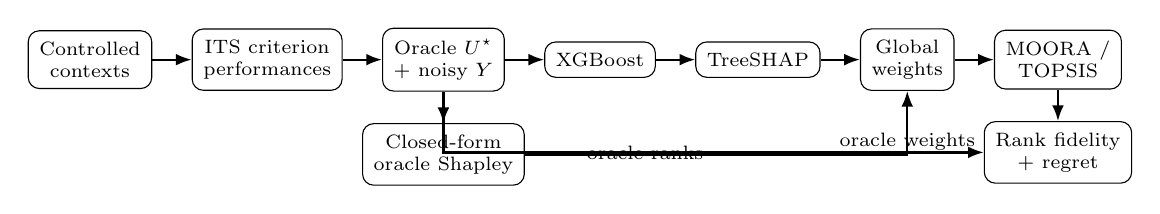
\begin{tikzpicture}[
node distance=4mm and 5mm,
box/.style={draw, rounded corners, align=center, inner sep=4pt, font=\scriptsize},
arr/.style={-{Latex[length=2mm]}, thick}
]
\node[box] (ctx) {Controlled\\contexts};
\node[box, right=of ctx] (perf) {ITS criterion\\performances};
\node[box, right=of perf] (oracle) {Oracle $U^\star$\\+ noisy $Y$};
\node[box, below=of oracle] (oshap) {Closed-form\\oracle Shapley};
\node[box, right=of oracle] (xgb) {XGBoost};
\node[box, right=of xgb] (shap) {TreeSHAP};
\node[box, right=of shap] (weights) {Global\\weights};
\node[box, right=of weights] (mcdm) {MOORA /\\TOPSIS};
\node[box, below=of mcdm] (metrics) {Rank fidelity\\+ regret};
\draw[arr] (ctx)--(perf);
\draw[arr] (perf)--(oracle);
\draw[arr] (oracle)--(xgb);
\draw[arr] (xgb)--(shap);
\draw[arr] (shap)--(weights);
\draw[arr] (weights)--(mcdm);
\draw[arr] (mcdm)--(metrics);
\draw[arr] (oracle)--(oshap);
\draw[arr] (oshap)-| node[pos=.75,below,font=\scriptsize]{oracle weights} (weights);
\draw[arr] (oracle) |- node[pos=.75,left,font=\scriptsize]{oracle ranks} (metrics);
\end{tikzpicture}%
}
\caption{Controlled prediction--attribution--weight-compression--decision pipeline.}
\label{fig:pipeline}
\end{figure}

\subsection{Context-Grouped Fit, Weight and Test Partitions}

Each seed generates $N_{\max}=1000$ contexts and one fixed random ordering. Consecutive blocks
of five are assigned three fit, one weight-calibration and one test position. The scarcity
subsets are nested prefixes:
\begin{equation}
\mathcal S_{25}\subset\mathcal S_{50}\subset\mathcal S_{100}
\subset\mathcal S_{250}\subset\mathcal S_{1000}.
\label{eq:nesting}
\end{equation}
Thus every $N$ has exactly 60/20/20 fit/weight/test proportions and a context never changes
partition when sample size increases. XGBoost and Ridge+ are fitted on fit contexts; TreeSHAP
background rows and oracle background moments also come from fit. Global SHAP/oracle weights,
permutation importance, CRITIC and entropy are estimated on weight-calibration contexts. Test
contexts are used only for final prediction and decision evaluation.

\subsection{XGBoost and TreeSHAP}

XGBoost models the noisy target $Y$ using the ten $g_j$ criteria \cite{chen2016xgboost}.
Hyperparameters and TreeSHAP background size are calibrated only on separate development seeds
and then frozen before the primary factorial experiment. Predictive performance is reported on
test contexts using $R^2$, MAE and RMSE; uncertainty is clustered/resampled at context level.

TreeSHAP uses `interventional' feature perturbation and fit-partition background rows. Its
global importance is averaged on the weight-calibration partition:
\begin{equation}
I_j^{SHAP}=\frac{1}{n_w}\sum_{i\in w}|\phi_{ij}^{XGB}|,
\qquad
w_j^{SHAP}=\frac{I_j^{SHAP}}{\sum_k I_k^{SHAP}}.
\label{eq:shapweights}
\end{equation}
Attribution recovery is measured by
\begin{align}
MAE_w&=\frac1p\sum_j|w_j^{SHAP}-w_j^\star|, \label{eq:maew}\\
TV_w&=\frac12\sum_j|w_j^{SHAP}-w_j^\star|, \label{eq:tvw}\\
\rho_w&=\operatorname{Spearman}(\mathbf w^{SHAP},\mathbf w^\star). \label{eq:spearmanw}
\end{align}
Top-3 and top-5 overlaps are also reported.

\subsection{Comparator Weights}

Table~\ref{tab:weightsmethods} summarises the primary weighting methods. All numerical safeguards
use $\eps=10^{-12}$.

\begin{table}[t]
\centering
\caption{Primary weighting methods and information used.}
\label{tab:weightsmethods}
\small
\begin{tabularx}{\linewidth}{@{}l c X@{}}
\toprule
\textbf{Method} & \textbf{Uses $Y$?} & \textbf{Primary definition}\\
\midrule
Oracle & -- & Mean absolute closed-form oracle Shapley on weight partition.\\
SHAP & Yes & Mean absolute interventional TreeSHAP on weight partition.\\
PI & Yes & 20-repeat context-block permutation importance on weight partition.\\
Ridge+ & Yes & Non-negative standardized ridge coefficients fitted on fit partition.\\
CRITIC & No & Contrast/conflict on min--max-normalised weight partition.\\
Entropy & No & Shannon diversification on min--max-normalised weight partition.\\
Equal & No & $w_j=1/p$.\\
\bottomrule
\end{tabularx}
\end{table}

For CRITIC and entropy, the weight-calibration matrix is first min--max normalised criterion by
criterion; effectively constant columns receive zero information content. CRITIC then uses
\begin{equation}
C_j=s_j\sum_k(1-r_{jk}),
\qquad
w_j^{CRITIC}=\frac{C_j}{\sum_lC_l}.
\label{eq:critic}
\end{equation}
Entropy uses $p_{ij}=\tilde g_{ij}/\sum_i\tilde g_{ij}$, the convention $0\log0=0$,
\begin{equation}
e_j=-\frac{1}{\log n_w}\sum_i p_{ij}\log p_{ij},
\qquad
w_j^{ENT}=\frac{1-e_j}{\sum_l(1-e_l)}.
\label{eq:entropy}
\end{equation}

Ridge+ solves, on standardized fit data,
\begin{equation}
\hat{\boldsymbol\beta}
=
\arg\min_{\boldsymbol\beta\ge0}
\left[\|\mathbf y-X\boldsymbol\beta\|_2^2
+\tau\|\boldsymbol\beta\|_2^2\right],
\qquad
w_j^{Ridge+}=\frac{\hat\beta_j}{\sum_k\hat\beta_k},
\label{eq:ridgeplus}
\end{equation}
with $\tau$ chosen by grouped CV within fit contexts. The non-negativity constraint avoids
turning a wrongly signed coefficient into a large positive weight by absolute value.

Permutation importance uses MSE and reassigns the complete six-alternative vector of one
criterion between weight-calibration contexts. Twenty permutations are averaged; negative mean
importances are truncated at zero before normalisation. If any data-driven method produces a
zero denominator, the implementation falls back to equal weights and records a diagnostic flag.

\subsection{MCDM and Direct-Model Decision Reference}

The primary downstream operator is weighted MOORA, applied to the same benefit-oriented matrix
$G_s=[g_{asj}]$. For each context,
\begin{equation}
r_{asj}=\frac{g_{asj}}{\sqrt{\sum_{a=1}^{6}g_{asj}^2}+\eps},
\qquad
S_{as}^{(q)}=\sum_{j=1}^{10}w_j^{(q)}r_{asj}.
\label{eq:moora}
\end{equation}
Alternatives are ranked by descending score. Classical TOPSIS is used as an aggregation
robustness check \cite{brauers2006moora,hwang1981topsis}.

The fitted XGBoost model is also used directly:
\begin{equation}
\hat a_s^{XGB}=\arg\max_a\hat Y_{as}.
\label{eq:directxgb}
\end{equation}
This is not an MCDM weighting method; it is a decision-information reference. If Direct-XGBoost
retains high decision fidelity while SHAP-weight MOORA does not, the information loss lies in
the attribution/global-weight/MCDM compression rather than prediction alone.

Random-weight diagnostics draw $K=200$ vectors from $Dirichlet(\mathbf1)$ per replication and
report the distribution of decision metrics. A modal-winner diagnostic chooses, from the
weight-calibration contexts only, the most frequent oracle-optimal alternative and evaluates
that constant Top-1 prediction on the test contexts.

% ============================================================
\section{Decision-Fidelity Diagnostics}
\label{sec:decision}
% ============================================================

The oracle-optimal alternative is
\begin{equation}
a_s^\star=\arg\max_aU_{as}^\star.
\label{eq:oraclechoice}
\end{equation}
Ranking agreement uses Kendall $\tau_b$ with a deterministic average-rank tie rule. Top-1
accuracy is
\begin{equation}
Acc_1^{(q)}
=\frac{1}{|\mathcal S_{test}|}
\sum_{s\in test}\I(\hat a_s^{(q)}=a_s^\star).
\label{eq:top1}
\end{equation}
The principal decision-theoretic loss is normalized oracle regret:
\begin{equation}
Regret_s^{(q)}
=
\frac{U_{a_s^\star,s}^\star-U_{\hat a_s^{(q)},s}^\star}
{\max_aU_{as}^\star-\min_aU_{as}^\star+\eps}.
\label{eq:regret}
\end{equation}
Mean, median and 95th-percentile regret are reported.

Near ties are quantified by the normalized oracle decision margin
\begin{equation}
M_s=
\frac{U_{(1),s}^\star-U_{(2),s}^\star}
{\max_aU_{as}^\star-\min_aU_{as}^\star+\eps}.
\label{eq:margin}
\end{equation}
Accuracy and regret are analysed conditional on $M_s$, distinguishing genuine method failure
from intrinsically ambiguous decisions.

Rather than claiming a strict additive error decomposition, the study reports a stage-wise
fidelity ladder:
\begin{align}
S_{as}^{main}&=\sum_j\alpha_jq_j(g_{asj}), \label{eq:stagemain}\\
S_{as}^{wq}&=\sum_jw_j^\star q_j(g_{asj}), \label{eq:stagewq}\\
S_{as}^{wg}&=\sum_jw_j^\star g_{asj}. \label{eq:stagewg}
\end{align}
These are compared sequentially with the full oracle $U^\star$, Oracle-weight MOORA,
SHAP-weight MOORA and Direct-XGBoost ranking. Adjacent differences are diagnostic contrasts,
not claimed to be an additive causal decomposition. One attribution-specific contrast is
\begin{equation}
\Delta\bar R_{attr}
=
\bar R^{SHAP\text{-}MOORA}-\bar R^{Oracle\text{-}MOORA}.
\label{eq:attrregret}
\end{equation}

% ============================================================
\section{Experimental Protocol}
\label{sec:experiment}
% ============================================================

\subsection{Primary Factorial Design}

The four primary factors are
\begin{align}
N&\in\{25,50,100,250,1000\}, & c&\in\{0.10,0.30,0.60\},\label{eq:factors1}\\
\rho&\in\{0,0.4,0.8\}, & \lambda&\in\{0,0.5,1\}.\label{eq:factors2}
\end{align}
The $5\times3\times3\times3=135$ conditions are repeated over 30 pre-specified primary seeds,
for 4050 primary replications. The reference condition is
\begin{equation}
(N,c,\rho,\lambda)=(250,0.30,0.4,0.5).
\label{eq:reference}
\end{equation}
Technology-response parameters and base criterion/target noise draws are sampled once per seed
and reused across factor levels. For each $(\rho,\lambda)$ cell, $s_U$ is calculated on the
full 1000-context master pool so that changing $N$ does not alter the imposed noise scale.
Realized SNR is logged for every cell.

\subsection{Alpha-Dispersion Stress Test}

Equal main-effect coefficients can make attribution magnitude heavily dispersion-driven in the
additive oracle. The primary heterogeneous vector in Eq.~\eqref{eq:alpha} avoids that special
case. At the reference condition, a secondary stress test uses the same coefficient multiset
and assigns it (i) according to the frozen neutral mapping, (ii) aligned with fit-partition
criterion dispersion, and (iii) anti-aligned with that dispersion. This directly tests whether
information-based weights benefit simply from coincidental alignment between dispersion and
outcome relevance.

\subsection{Mandatory Pilot and Degeneracy Checks}

Before the full factorial experiment, the reference condition is run on reserved development
seeds. Mandatory diagnostics include realized criterion ranges and clipping rates, oracle-signal
SD and SNR, the number of distinct oracle winners, modal winner share, normalized winner
entropy, the decision-margin distribution, and the random-weight decision-metric distribution.
If structured methods are indistinguishable from random weights or one alternative dominates
nearly all contexts, the full grid is not launched; the generator must be revised transparently,
versioned and re-frozen before primary execution.

\subsection{Bootstrap, Shift and Robustness}

At the reference condition, $B=200$ context-level bootstrap replications resample fit and
weight-calibration contexts separately, refit the model, recompute attributions/weights and
evaluate on the fixed original test contexts \cite{efron1993bootstrap}. Confidence intervals
are reported for criterion weights, $TV_w$, Kendall $\tau_b$, Top-1 accuracy and regret. No
global cross-context probability that a particular ITS is rank 1 is reported.

A 50-generator ensemble varies $\boldsymbol\alpha$, nonlinearities and semantically admissible
interaction pairs; relative noise is recalibrated to each generator's signal SD. Two
out-of-distribution tests hold out the upper 20\% of demand pressure or the lower 20\% of
infrastructure readiness, with the remaining 80\% divided into fit and weight-calibration
partitions. Criterion-removal, $\pm10/20/30\%$ SHAP-weight perturbations, leave-one-alternative-
out analysis and MOORA--TOPSIS comparison provide secondary robustness checks.

\subsection{Statistical Analysis and Reproducibility}

Factor effects are summarized with repeated-seed regression/mixed-effects models using effect
sizes and uncertainty intervals rather than binary significance alone. Method comparisons are
paired because all methods share the same generated benchmark instances.

The protocol is frozen in a version-controlled specification before primary execution.
The repository records seeds, configurations, package versions, the Git commit, runtime and peak
memory. A TreeSHAP--XGBoost smoke test verifies local accuracy before the main pipeline is
implemented, and closed-form oracle Shapley is checked against exhaustive coalition enumeration.
When replications are parallelized externally, XGBoost uses one internal worker to avoid thread
oversubscription.

% ============================================================
\section{Results}
\label{sec:results}
% ============================================================

\ifresultsavailable
% The production pipeline should generate the following files or equivalent
% LaTeX-ready tables/figures. These paths are intentionally not read while
% \resultsavailablefalse.
%
% \input{results/tables/predictive_and_direct_xgb.tex}
% \input{results/tables/weight_recovery.tex}
% \input{results/tables/decision_fidelity.tex}
% \input{results/tables/factorial_summary.tex}
% \input{results/tables/alpha_alignment.tex}
% \input{results/tables/bootstrap_summary.tex}
%
% \begin{figure}[t]
% \centering
% \includegraphics[width=\linewidth]{results/figures/validity_boundaries.pdf}
% \caption{Validity boundaries across scarcity, dependence, relative noise and interaction strength.}
% \label{fig:validity}
% \end{figure}
%
% \begin{figure}[t]
% \centering
% \includegraphics[width=\linewidth]{results/figures/stagewise_fidelity.pdf}
% \caption{Stage-wise decision fidelity from oracle utility to learned-weight MCDM.}
% \label{fig:stages}
% \end{figure}
\else
\noindent\textit{Working-manuscript note.} Numerical results are intentionally omitted until the
version-controlled computational protocol has been executed. The submitted manuscript will
contain the generated predictive, attribution and decision-fidelity tables and figures; no
placeholder values will be submitted.
\fi

% ============================================================
\section{Discussion and Threats to Validity}
\label{sec:discussion}
% ============================================================

The benchmark is designed so that several outcomes are scientifically informative. SHAP may
recover oracle attribution and produce low regret across broad regimes; it may work only above
identifiable sample-quality thresholds; or simpler methods such as Ridge+ or even equal weights
may be equally competitive. A particularly informative outcome would be high Direct-XGBoost
decision fidelity together with poor SHAP-weight MOORA fidelity, indicating that useful
predictive information is lost when nonlinear/local structure is compressed into a single
global weight vector.

Several limitations are intentional. First, the capability mask and response bands are
literature-informed structural assumptions rather than empirical impact estimates. Second, the
Gaussian copula controls dependence but is not a calibrated urban joint distribution. Third,
interventional SHAP answers a particular feature-removal question and does not identify causal
effects. Fourth, oracle attribution weights are internal reference quantities rather than
stakeholder preferences. Fifth, the downstream MCDM operator itself introduces information loss;
this is why Oracle-weight MOORA and the stage-wise ladder are reported. Sixth, permutation
importance may become unreliable under strong predictor dependence because permutation can
force extrapolation \cite{hooker2021permutation}.

The synthetic ITS ranking therefore has no direct policy interpretation. A later empirical
extension can replace the context generator with measured traffic states and the technology-
response layer with calibrated SUMO/TraCI or field evidence, while retaining the same fidelity
audit. Expert/stakeholder weights would then enter as a separate normative comparator rather
than being treated as equivalent to predictive attribution.

% ============================================================
\section{Conclusion}
\label{sec:conclusion}
% ============================================================

This paper develops a controlled benchmark for testing the transition from predictive
importance to decision weights in ITS prioritisation. The methodological contribution lies not
in combining XGBoost, SHAP and MOORA, but in evaluating whether attribution fidelity survives
compression into a global criterion-weight vector and downstream decision rule. Closed-form
oracle interventional Shapley values, signal-relative noise, paired scarcity/dependence stress
tests, fair supervised and unsupervised baselines, Direct-XGBoost ranking and decision regret
make it possible to identify where the transition succeeds and where it breaks down. The final
claims will be determined by the pre-specified numerical experiment rather than by a desired
winner.

% ============================================================
\begin{thebibliography}{99}

\bibitem{chen2016xgboost}
Chen, T., Guestrin, C.:
XGBoost: A scalable tree boosting system.
In: Proceedings of the 22nd ACM SIGKDD International Conference on Knowledge Discovery and
Data Mining, pp. 785--794 (2016).
\url{https://doi.org/10.1145/2939672.2939785}

\bibitem{lundberg2017shap}
Lundberg, S.M., Lee, S.-I.:
A unified approach to interpreting model predictions.
In: Advances in Neural Information Processing Systems, vol. 30 (2017).

\bibitem{lundberg2020trees}
Lundberg, S.M., Erion, G., Chen, H., et al.:
From local explanations to global understanding with explainable AI for trees.
Nature Machine Intelligence \textbf{2}, 56--67 (2020).
\url{https://doi.org/10.1038/s42256-019-0138-9}

\bibitem{kumar2020shapleyproblems}
Kumar, I.E., Venkatasubramanian, S., Scheidegger, C., Friedler, S.:
Problems with Shapley-value-based explanations as feature importance measures.
In: Proceedings of the 37th International Conference on Machine Learning,
PMLR \textbf{119}, 5491--5500 (2020).

\bibitem{covert2020sage}
Covert, I., Lundberg, S.M., Lee, S.-I.:
Understanding global feature contributions with additive importance measures.
In: Advances in Neural Information Processing Systems, vol. 33 (2020).

\bibitem{janzing2020causal}
Janzing, D., Minorics, L., Bl{\"o}baum, P.:
Feature relevance quantification in explainable AI: A causal problem.
In: Proceedings of the 23rd International Conference on Artificial Intelligence and Statistics,
PMLR \textbf{108}, 2907--2916 (2020).

\bibitem{aas2021dependent}
Aas, K., Jullum, M., L{\o}land, A.:
Explaining individual predictions when features are dependent: More accurate approximations to
Shapley values.
Artificial Intelligence \textbf{298}, 103502 (2021).
\url{https://doi.org/10.1016/j.artint.2021.103502}

\bibitem{hooker2021permutation}
Hooker, G., Mentch, L., Zhou, S.:
Unrestricted permutation forces extrapolation: Variable importance requires at least one more
model, or there is no free variable importance.
Statistics and Computing \textbf{31}, 82 (2021).
\url{https://doi.org/10.1007/s11222-021-10057-z}

\bibitem{liu2021xaibench}
Liu, Y., Khandagale, S., White, C., Neiswanger, W.:
Synthetic benchmarks for scientific research in explainable machine learning.
Proceedings of the Neural Information Processing Systems Track on Datasets and Benchmarks
\textbf{1} (2021).

\bibitem{agarwal2022openxai}
Agarwal, C., Krishna, S., Saxena, E., Pawelczyk, M., Johnson, N., Puri, I., Zitnik, M.,
Lakkaraju, H.:
OpenXAI: Towards a transparent evaluation of model explanations.
In: Advances in Neural Information Processing Systems, vol. 35, Datasets and Benchmarks Track
(2022).

\bibitem{lee2025xaiunits}
Lee, J.R., Emami, S., Hollins, M.D., Wong, T.C.H., Villalobos S\'anchez, C.I., Toni, F.,
Zhang, D., Dejl, A.:
XAI-Units: Benchmarking explainability methods with unit tests.
arXiv:2506.01059 (2025).

\bibitem{ciano2025xaimcdm}
Ciano, T., Ferrara, M.:
Explainable multi-criteria decision making for tourism economics: Integrating XAI with MCDM for
a robust accommodation performance assessment.
Decisions in Economics and Finance (2025).
\url{https://doi.org/10.1007/s10203-025-00553-6}

\bibitem{demir2025shapmultimoora}
Demir, A.S., Da{\u g}deviren, U., Kurnaz, T.F., Erden, C., K{\"o}k{\c c}am, A.H.:
An integrated SHAP-MCDM approach for slope stability prediction based on machine learning
algorithms.
Natural Hazards \textbf{121}(18), 21811--21836 (2025).
\url{https://doi.org/10.1007/s11069-025-07665-7}

\bibitem{zakeri2024mlmcdm}
Zakeri, S., Konstantas, D., Sorooshian, S., Chatterjee, P.:
A novel ML-MCDM-based decision support system for evaluating autonomous vehicle integration
scenarios in Geneva's public transportation.
Artificial Intelligence Review \textbf{57}, 310 (2024).
\url{https://doi.org/10.1007/s10462-024-10917-w}

\bibitem{sudakov2026weights}
Sudakov, V.A., Timoshenko, A.V., Komarova, L.A., Zakharov, A.S.:
Automation of determining criterion weights in decision support tasks based on regression
analysis results.
Mathematics \textbf{14}(13), 2412 (2026).
\url{https://doi.org/10.3390/math14132412}

\bibitem{diakoulaki1995critic}
Diakoulaki, D., Mavrotas, G., Papayannakis, L.:
Determining objective weights in multiple criteria problems: The CRITIC method.
Computers \& Operations Research \textbf{22}(7), 763--770 (1995).
\url{https://doi.org/10.1016/0305-0548(94)00059-H}

\bibitem{shannon1948}
Shannon, C.E.:
A mathematical theory of communication.
Bell System Technical Journal \textbf{27}, 379--423, 623--656 (1948).

\bibitem{brauers2006moora}
Brauers, W.K.M., Zavadskas, E.K.:
The MOORA method and its application to privatization in a transition economy.
Control and Cybernetics \textbf{35}(2), 445--469 (2006).

\bibitem{hwang1981topsis}
Hwang, C.-L., Yoon, K.:
Multiple Attribute Decision Making: Methods and Applications.
Springer, Berlin (1981).

\bibitem{efron1993bootstrap}
Efron, B., Tibshirani, R.J.:
An Introduction to the Bootstrap.
Chapman \& Hall/CRC, New York (1993).

\bibitem{fhwa2016corridors}
Federal Highway Administration:
Planning for Transportation Systems Management and Operations Within Corridors: A Desk
Reference, FHWA-HOP-16-037 (2016).
\url{https://ops.fhwa.dot.gov/Publications/fhwahop16037/}

\bibitem{fhwa2017atm}
Kuhn, B., Balke, K., Wood, N.:
Active Traffic Management (ATM) Implementation and Operations Guide.
FHWA-HOP-17-056, Federal Highway Administration (2017).
\url{https://ops.fhwa.dot.gov/publications/fhwahop17056/}

\bibitem{usdotv2x}
U.S. Department of Transportation, ITS Joint Program Office:
V2X Applications and Use Cases.
\url{https://its.dot.gov/research-areas/V2X-Deployment/overview/v2x-applications/}
(accessed 13 August 2026).

\end{thebibliography}

\end{document}
